\documentclass[fleqn,10pt]{article}

\usepackage{multirow}
\usepackage{float}
\usepackage{array}
\usepackage{dirtytalk}
\usepackage{csquotes}
\usepackage{amsmath}
\usepackage{graphicx}
\usepackage{amssymb}
\usepackage{pifont}

\usepackage{natbib}
%\bibliographystyle{agsm}
\bibliographystyle{named}
\let\hardvardurl\url
\usepackage{url}
\usepackage[breaklinks]{hyperref}

\newcommand{\cmark}{\ding{51}}%
\newcommand{\xmark}{\ding{53}}%

\title{Assessing Gender Bias in Machine Translation -- A Case Study with Google Translate}

\begin{document}

\maketitle

\begin{abstract}
Recently there has been a growing concern in academia, industrial research labs and the mainstream commercial media about the phenomenon dubbed as \emph{machine bias}, where trained statistical models -- unbeknownst to their creators -- grow to reflect controversial societal asymmetries, such as gender or racial bias. A significant number of Artificial Intelligence tools have recently been suggested to be harmfully biased towards some minority, with reports of racist criminal behavior predictors, Apple's Iphone X failing to differentiate between two distinct Asian people and the now infamous case of Google photos' mistakenly classifying people of color as gorillas. Although a systematic study of such biases can be difficult, we believe that automated translation tools can be exploited through gender neutral languages to yield a window into the phenomenon of gender bias in AI.

In this paper, we obtained a comprehensive list of job positions from the U.S. Bureau of Labor Statistics and used it to build sentences in the format of \say{He/She is an Engineer} in 11 different gender neutral languages such as Hungarian, Chinese, Yoruba, etc. We translate these sentences into English using the Google Translate API, and collect statistics about the frequency of female, male and gender-neutral pronouns in the translated output. We then show that Google Translate exhibits a strong tendency towards male defaults, which is exaggerated for fields suggested to be troubled with gender stereotypes such as STEM (Science, Technology, Engineering and Mathematics) jobs. We ran these statistics against BLS' data for the frequency of female participation in each job position, in which we show that Google Translate fails to reproduce the real-world distribution of female workers. In summary, we provide evidence that even if one does not expect in principle a 50:50 pronominal gender distribution, Google Translate yields male defaults much more frequently than what would be expected from demographic data alone.

We believe that our study can shed further light on the phenomenon of machine bias and are hopeful that it will ignite a debate about the need for augmented current statistical translation tools with debiasing techniques -- which can already be found in the scientific literature.
\end{abstract}

\section{Introduction}

Although the idea of automated translation can in principle be traced back to as long as the 17th century with Ren\'{e} Descartes proposal of an \say{universal language} \cite{dascal1982universal}, machine translation has only existed as a technological field since the 1950s, with a pioneering memorandum by  Warren Weaver \cite{locke1955machine,weaver1955translation} discussing the possibility of employing digital computers to perform automated translation. The now famous Georgetown-IBM experiment followed not long after, providing the first experimental demonstration of the prospects of automating translation by the means of successfully converting more than sixty Russian sentences into English \cite{gordin2015scientific}. Early systems improved upon the results of the Georgetown-IBM experiment by exploiting Noam Chomsky's theory of generative linguistics, and the field experienced a sense of optimism about the prospects of fully automating natural language translation. As is customary with artificial intelligence, the initial optimistic stage was followed by an extended period of strong disillusionment with the field, of which the catalyst was the influential 1966 ALPAC (Automatic Language Processing Advisory Committee) report( \cite{hutchins1986machine}. 
Such research was then disfavoured in the United States, making a re-entrance in the 1970s before the 1980s surge in statistical methods for machine translation \cite{koehn2009statistical,Moses2007}. Statistical and example-based machine translation have been on the rise ever since \cite{Bahdanau2014,carl2003recent,Firat2017}, with highly successful applications such as Google Translate (recently ported to a neural translation technology \cite{wu2016google}) amounting to over $200$ million users daily.

In spite of the recent commercial success of automated translation tools (or perhaps stemming directly from it), machine translation has amounted a significant deal of criticism. Noted philosopher and founding father of generative linguistics Noam Chomsky has argued that the achievements of machine translation, while successes in a particular sense, are \emph{not successes in the sense that science has ever been interested in}: they merely provide effective ways, according to Chomsky, of approximating unanalyzed data \cite{Chomsky2011,norvig2017chomsky}. Chomsky argues that the faith of the MT community in statistical methods is absurd by analogy with a standard scientific field such as physics \cite{Chomsky2011}:

\begin{quotation}
\textsl{I mean actually you could do physics this way, instead of studying things like balls rolling down frictionless planes, which can't happen in nature, if you took a ton of video tapes of what's happening outside my office window, let's say, you know, leaves flying and various things, and you did an extensive analysis of them, you would get some kind of prediction of what's likely to happen next, certainly way better than anybody in the physics department could do. Well that's a notion of success which is I think novel, I don't know of anything like it in the history of science}.
\end{quotation}

Leading AI researcher and Google's Director of Research Peter Norvig responds to these arguments by suggesting that even standard physical theories such as the Newtonian model of gravitation are, in a sense, \emph{trained} \cite{norvig2017chomsky}:

\begin{quotation}
\textsl{As another example, consider the Newtonian model of gravitational attraction, which says that the force between two objects of mass $m_1$ and $m_2$ a distance $r$ apart is given by}
\begin{equation*}
F = G m_1 m_2 / r^2
\end{equation*}
\textsl{where $G$ is the universal gravitational constant. This is a trained model because the gravitational constant G is determined by statistical inference over the results of a series of experiments that contain stochastic experimental error. It is also a deterministic (non-probabilistic) model because it states an exact functional relationship. I believe that Chomsky has no objection to this kind of statistical model. Rather, he seems to reserve his criticism for statistical models like Shannon's that have quadrillions of parameters, not just one or two.}
\end{quotation}

Chomsky and Norvig's debate \cite{norvig2017chomsky} is a microcosmos of the two leading standpoints about the future of science in the face of increasingly sophisticated statistical models. Are we, as Chomsky seems to argue, jeopardizing science by relying on statistical tools to perform predictions instead of perfecting traditional science models, or are these tools, as Norvig argues, components of the scientific standard since its conception? Currently there are no satisfactory resolutions to this conundrum, but perhaps statistical models pose an even greater and more urgent threat to our society. 

On a 2014 article, Londa Schiebinger suggested that scientific research fails to take gender issues into account, arguing that the phenomenon of male defaults on new technologies such as Google Translate provides a window into this asymmetry \cite{schiebinger2014scientific}. Since then, recent worrisome results in machine learning have somewhat supported Schiebinger's view. Not only Google photos' statistical image labeling algorithm has been found to classify dark-skinned people as gorillas \cite{garcia2016racist} and purportedly intelligent programs have been suggested to be negatively biased against black prisoners when predicting criminal behavior \cite{angwin2016machine} but the machine learning revolution has also indirectly revived heated debates about the controversial field of physiognomy, with proposals of AI systems capable of identifying the sexual orientation of an individual through its facial characteristics \cite{wang2017deep}. Similar concerns are growing at an unprecedented rate in the media, with reports of Apple's Iphone X face unlock feature failing to differentiate between two different Asian people \cite{womanunlockphone2017} and automatic soap dispensers which reportedly do not recognize black hands \cite{racistsoapdispenser2017}. \emph{Machine bias}, the phenomenon by which trained statistical models unbeknownst to their creators grow to reflect controversial societal assymetries, is growing into a pressing concern for the modern times, invites us to ask ourselves whether there are limits to our dependence on these techniques -- and more importantly, whether some of these limits have already been traversed. In the wave of algorithmic bias, some have argued for the creation of some kind of agency in the likes of the Food and Drug Administration, with the sole purpose of regulating algorithmic discrimination \cite{kirkpatrick2016battling}.

With this in mind, we propose a quantitative analysis of the phenomenon of gender bias in machine translation. We illustrate how this can be done by simply exploiting Google Translate to map sentences from a gender neutral language into English. As Figure \ref{fig:screenshot-gtranslate-hungarian} exemplifies, this approach produces results consistent with the hypothesis that sentences about stereotypical gender roles are translated accordingly with high probability: \emph{nurse} and \emph{baker} are translated with female pronouns while \emph{engineer} and \emph{CEO} are translated with male ones.

\begin{figure}[h]
	\centering
	\fbox{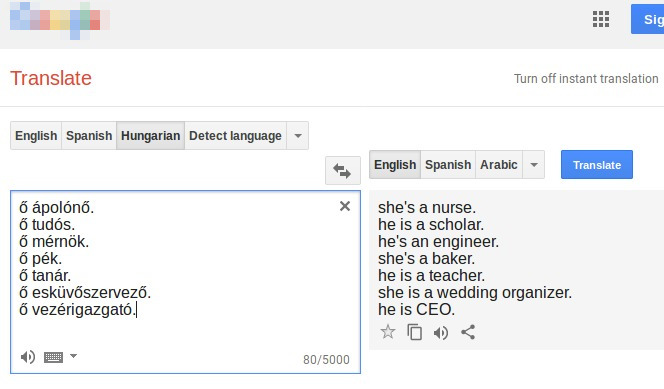
\includegraphics[width=\linewidth]{pictures/screenshot-gtranslate-hungarian}}
	\caption{Translating sentences from a gender neutral language such as Hungarian to English provides a glimpse into the phenomenon of gender bias in machine translation. This screenshot from Google Translate shows how occupations from traditionally male-dominated fields such as scholar, engineer and CEO are interpreted as male, while occupations such as nurse, baker and wedding organizer are interpreted as female.}
	\label{fig:screenshot-gtranslate-hungarian}
\end{figure}

\section{Motivation}

As of 2017, Google translate is one of the largest publicly available machine translation tools in existence, amounting 200 million users daily \cite{Gtranslate200daily2017}. Initially relying on United Nations and European Parliament transcripts to gather data, since 2014 Google Translate has inputed content from its users through the Translate Community initiative \cite{TranslateCommunity}. Recently however there has been a growing concern about gender asymmetries in the translation mechanism, with some heralding it as \say{sexist} \cite{AlgorithmGtranslateSexist2018}. This concern has to at least some extent a scientific backup: A recent study has shown that word embeddings are particularly prone to yielding gender stereotypes \cite{bolukbasi2016man}. Fortunately, the researchers propose a relatively simple \emph{debiasing} algorithm with promising results: they were able to cut the proportion of stereotypical analogies from $19\%$ to $6\%$ without any significant compromise in the performance of the word embedding technique. They are not alone: there is a growing effort to systematically discover and resolve issues of algorithmic bias in black-box algorithms \cite{hajian2016algorithmic} The success of these results suggest that a similar technique could be used to remove gender bias from Google Translate outputs, should it exist. This paper intends to investigate whether it does. We are optimistic that our research endeavors can be used to argue that there is a positive payoff in redesigning modern statistical translation tools.

\section{Assumptions and Preliminaries}

\section{Materials and Methods}

% The hungarian punctuation in 'ő' is not rendered in the PDF. This needs to be fixed somehow. The same problem extends to Table 4 (label tab:templates)
We shall assume and then show that the phenomenon of gender bias in machine translation can be assessed by mapping sentences constructed in gender neutral languages to English by the means of an automated translation tool. Specifically, we can translate sentences such as the Hungarian \say{ő ápolónő}, where \say{ápolónő} translates to \say{nurse} and \say{ő} is a gender-neutral pronoun meaning either he, she or it, to English, yielding in this example the result \say{she's a nurse} on Google Translate. As Figure \ref{fig:screenshot-gtranslate-hungarian} clearly shows, the same template yields a male pronoun when \say{nurse} is replaced by \say{engineer}. The same basic template can be ported to all other gender neutral languages, as Table \ref{tab:templates} shows. Given the success of Google Translate, which amounts to 200 million users daily, we have chosen to exploit its API to obtain the desired thermometer of gender bias. Also, in order to solidify our results, we have decided to work 
% PEDRO: Removed "with as many gender neutral languages as possible"
 with a fair amount of gender neutral languages, forming a list of these with help from the World Atlas of Language Structures \cite{wals} and other sources. Table \ref{tab:gender-neutral-languages} compiles all languages we chose to use, with additional columns informing whether they
(1) exhibit a pronominal gender system and (2) are supported by Google Translate. Because pronominal gender systems defy the purposes of our technique, such languages have been discarded.

There is a prohibitively large class of nouns and adjectives that could in principle be substituted in the templates of Table \ref{tab:templates}. To simplify our dataset, we have decided to obtain a comprehensive list of professional occupations, which, we believe, are an interesting window into the nature of gender bias. This time we resorted to using the Bureau of Labor Statistics' detailed occupations table \cite{BLS2017}, from the United States Department of Labor, for providing such a list. The values inside, however, had to be expanded since each line contained multiple occupations and sometimes very specific ones. Fortunately this table also provided a percentage of women participation in the jobs shown, for those that had more than 50 thousand workers. We then separated the curated jobs into categories (Artistic, Corporate, Theatre, etc.) as shown in Table \ref{tab:occupations}. Finally, Table \ref{tab:occupations-examples} shows thirty examples of randomly selected occupations from our dataset. Finally, we have selected a small list of 21 adjectives, presented in Table \ref{tab:adjectives}.

% Table containing a list of gender neutral languages with information about pronominal gender systems and GTranslate support
\begin{table}[H]
\begin{small}
	\centering
	\begin{tabular}{|c|m{2cm}|m{2cm}|c|c|}
	\hline
	Language Family 				& Language 				& Pronominal Gender System 	& Supported 	& Tested 		\\ \hline \hline
	\multirow{2}{*}{Austronesian} 	& Malay 				& \xmark 					& \checkmark	& \checkmark	\\
									& Tagalog 				& \xmark 					& \xmark		& \xmark		\\ \hline
	\multirow{3}{*}{Finno-Ugric} 	& Estonian 				& \xmark 					& \checkmark 	& \checkmark	\\
									& Finnish 				& \xmark 					& \checkmark	& \checkmark	\\
									& Hungarian 			& \xmark 					& \checkmark 	& \checkmark	\\ \hline
	\multirow{4}{*}{Indo-European} 	& Armenian 				& \xmark 					& \checkmark 	& \checkmark	\\
									& Bengali 				& \xmark 					& \checkmark 	& \xmark		\\
									& English 				& \checkmark 				& \checkmark 	& \xmark 		\\
									& Persian 				& \checkmark 				& \checkmark 	& \xmark 		\\ \hline
	\multirow{3}{*}{Indo-Aryan} 	& Maithili 				& \xmark 					& \xmark 		& \xmark 		\\
									& Nepali 				& \xmark 					& \checkmark	& \xmark		\\
									& Oriya 				& \xmark 					& \xmark 		& \xmark 		\\ \hline
	\multirow{10}{*}{} 				& Japanese 				& \xmark 					& \checkmark 	& \checkmark	\\
									& Korean 				& O 						& \checkmark 	& \xmark		\\
									& Turkish 				& \xmark 					& \checkmark 	& \checkmark	\\
									& Yoruba 				& \xmark 					& \checkmark 	& \checkmark	\\
									& Basque 				& \xmark 					& \checkmark 	& \checkmark	\\
									& Swahili 				& \xmark 					& \checkmark 	& \checkmark	\\
									& Chinese 				& O 						& \checkmark 	& \checkmark	\\
									& Cantonese 			& \xmark 					& \xmark		& \xmark		\\
									& Pipil 				& \xmark 					& \xmark		& \xmark		\\
									& Quechuan 				& \xmark 					& \xmark		& \xmark		\\ \hline
	\multirow{4}{*}{Constructed} 	& Esperanto 			& \checkmark 				& \checkmark 	& \xmark		\\
									& Ido 					& O 						& \xmark 		& \xmark 		\\ \cline{2-2}
									& Lingua Franca Nova 	& \xmark 					& \xmark 		& \xmark 		\\ \cline{2-2}
									& Interlingua 			& \xmark 					& \xmark 		& \xmark 		\\ \hline
	\end{tabular}
	\caption{Selected gender neutral languages obtained from the Wikipedia article \url{https://en.wikipedia.org/wiki/Gender_neutrality_in_genderless_languages}. Languages are grouped according to language families and classified according to whether they exhibit pronominal gender system (\checkmark: yes, \xmark:~no, O: it is optional). For the purposes of this work, we have decided to work only with languages lacking such a system and, as such, Persian and Esperanto have been discarded. Languages lacking support from Google Translate have been discarded.}
	\label{tab:gender-neutral-languages}
	\end{small}
\end{table}

% List of occupation categories obtained from the U.S. Bureau of Labor Statistics, with nº of occupations per category and female participation (%) in each category
\begin{table}[H]
\begin{small}
	\centering
	\begin{tabular}{|m{3.5cm}|c|c|c|}
	\hline	
	Category 										& Group 						& \# Occupations 	& Female Participation	\\ \hline \hline
	Education, training, and library 				& Education						& $22$ 				& $73.0\%$				\\ \hline
	Business and financial operations				& Corporate						& $46$ 				& $54.0\%$				\\ \hline
	Office and administrative support				& Service						& $87$ 				& $72.2\%$				\\ \hline
	Healthcare support 								& Healthcare					& $16$ 				& $87.1\%$				\\ \hline
	Management 										& Corporate						& $46$ 				& $39.8\%$				\\ \hline
	Installation, maintenance, and repair 			& Service						& $91$ 				& $4.0\%$ 				\\ \hline
	Healthcare practitioners and technical 			& Healthcare					& $43$ 				& $75.0\%$				\\ \hline
	Community and social service 					& Service						& $14$ 				& $66.1\%$				\\ \hline
	Sales and related 								& Corporate						& $28$ 				& $49.1\%$				\\ \hline
	Production 										& Production					& $264$ 			& $28.9\%$				\\ \hline
	Architecture and engineering 					& STEM 							& $29$ 				& $16.2\%$				\\ \hline
	Life, physical, and social science				& STEM 							& $34$ 				& $47.4\%$				\\ \hline
	Transportation and material moving				& Service						& $70$ 				& $17.3\%$				\\ \hline
	Arts, design, entertainment, sports, and media 	& Arts / Entertainment 			& $37$ 				& $46.9\%$				\\ \hline
	Legal											& Legal 						& $7$				& $52.8\%$				\\ \hline
	Protective Service 								& Service 						& $28$ 				& $22.3\%$				\\ \hline
	Food preparation and serving related 			& Service 						& $17$ 				& $53.8\%$				\\ \hline
	Farming, fishing, and forestry 					& Farming / Fishing / Forestry 	& $13$ 				& $23.4\%$				\\ \hline
	Computer and mathematical						& STEM 							& $16$ 				& $25.5\%$				\\ \hline
	Personal care and service						& Service 						& $33$ 				& $76.1\%$				\\ \hline
	Construction and extraction 					& Construction / Extraction 	& $68$ 				& $3.0\%$ 				\\ \hline
	Building and grounds cleaning and maintenance 	& Service 						& $10$ 				& $40.7\%$				\\ \hline \hline
	Total											& - 							& $1019$			& $41.3\%$				\\ \hline
	\end{tabular}
	\caption{Selected occupations obtained from the U.S. Bureau of Labor Statistics \url{https://???}, grouped by category. We obtained a total of $1019$ occupations from $22$ distinct categories. We have further grouped them into broader groups (or \emph{super-categories}) to ease analysis and visualization.}
	\label{tab:occupations}
	\end{small}
\end{table}

% List of sentence templates for assessing gender bias in the translation from source language to English
\begin{table}[H]
\small{
	\centering
	\begin{tabular}{|c|c|}
	\hline
	Language 	& Sentence template 						\\ \hline \hline
	Malay		& dia adalah $\langle occupation \rangle$ 	\\ \hline
	Estonian	& ta on $\langle occupation \rangle$ 		\\ \hline
	Finnish		& hän on $\langle occupation \rangle$ 		\\ \hline
	Hungarian	& ő $\langle occupation \rangle$ 			\\ \hline
	Armenian	& na $\langle occupation \rangle$ e 		\\ \hline
	Japanese	& $\langle occupation \rangle$ です			\\ \hline
	Turkish		& o bir $\langle occupation \rangle$ 		\\ \hline
	Yoruba		& o jẹ $\langle occupation \rangle$ 		\\ \hline
	Basque		& $\langle occupation \rangle$ da 			\\ \hline
	Swahili		& yeye ni $\langle occupation \rangle$ 		\\ \hline
	Chinese		& ta $\langle occupation \rangle$ 			\\ \hline
	\end{tabular}
	\caption{Templates used to infer gender biases in the translation to the English language.}
	\label{tab:templates}
	}
\end{table}

% Table with a random sample of 30 occupations obtained from the U.S. Bureau of Labor Statistics
\begin{table}[H]
\small{
	\centering
	\begin{tabular}{|c|c|c|c|c|}
	\hline
	Insurance sales agent 	& Editor 						& Rancher 					\\ \hline
	Ticket taker 			& Pile-driver operator 			& Tool maker 				\\ \hline
	Jeweler 				& Judicial law clerk 			& Auditing clerk 			\\ \hline
	Physician 				& Embalmer 						& Door-to-door salesperson 	\\ \hline
	Packer 					& Bookkeeping clerk 			& Community health worker 	\\ \hline
	Sales worker 			& Floor finisher 				& Social science technician \\ \hline
	Probation officer 		& Paper goods machine setter 	& Heating installer 		\\ \hline
	Animal breeder 			& Instructor 					& Teacher assistant 		\\ \hline
	Statistical assistant 	& Shipping clerk 				& Trapper 					\\ \hline
	Pharmacy aide 			& Sewing machine operator 		& Service unit operator 	\\ \hline
	\end{tabular}
	\caption{A randomly selected example subset of thirty occupations obtained from our dataset with a total of $1019$ different occupations.}
	\label{tab:occupations-examples}
	}
\end{table}

% Table with all adjectives we experimented with
\begin{table}[H]
\small{
	\centering
	\begin{tabular}{|c|c|c|}
	\hline
	Happy 		& Sad 		& Right 	\\ \hline
	Wrong 		& Afraid	& Brave 	\\ \hline
	Smart		& Dumb		& Proud 	\\ \hline
	Ashamed		& Kind		& Cruel 	\\ \hline
	Envious		& Loving	& Hateful 	\\ \hline
	Modest 		& Arrogant	& Guilty	\\ \hline
	Innocent	& Helpless	& Shy		\\ \hline
	\end{tabular}
	\caption{Adjectives}
	\label{tab:adjectives}
	}
\end{table}

\section{Distribution of translated gender pronouns per occupation category}

A sensible way to group translation data is to coalesce occupations in the same category and collect statistics about how prominent male defaults are in each field. What we have found is that Google Translate does indeed translate sentences with male pronouns with greater probability 
% Add statistical test here
than it does either female or gender-neutral pronouns. Furthermore, this bias is seemingly aggravated for fields suggested to be troubled by male stereotypes,
% Add reference here
such as life and physical sciences, architecture, engineering, computer science and mathematics. Table \ref{tab:gender-by-category} summarizes these data, and Table \ref{tab:gender-by-category-grouped} summarizes it even further by coalescing occupation categories into broader groups to ease interpretation. For instance, STEM (Science, Technology, Engineering and Mathematics) fields are grouped into a single category, which helps us compare the large asymmetry between gender pronouns in these fields ($80.322\%$ of male defaults) to that of more evenly distributed fields such as healthcare ($59.014\%$).

% Table with our gender bias results grouped by category
\begin{table}[H]
\small{
	\centering
	\begin{tabular}{|c|c|c|c|}
	\hline
	Category 								& Female ($\%$)	& Male ($\%$)	& Neutral ($\%$) \\ \hline
	\hline		
	Education / Training / Library 			& $23.737$ 		& $58.081$		& $3.535$		\\ \hline
	Business / Financial 					& $6.039$		& $62.319$		& $8.937$		\\ \hline
	Office / Administrative					& $9.962$		& $56.322$		& $9.451$		\\ \hline
	Healthcare support						& $27.083$		& $50.000$		& $9.722$		\\ \hline
	Management								& $11.594$		& $61.111$		& $4.831$		\\ \hline
	Installation / Maintenance / Repair		& $3.297$		& $62.393$		& $14.164$		\\ \hline
	Healthcare practitioners / technical	& $18.088$		& $61.499$		& $8.527$		\\ \hline
	Community and social service			& $14.286$ 		& $60.317$		& $5.556$		\\ \hline
	Sales and related						& $7.540$		& $64.683$		& $10.714$		\\ \hline
	Production								& $15.32$		& $45.370$		& $15.825$		\\ \hline
	Architecture and engineering			& $1.916$		& $75.862$		& $6.130$		\\ \hline
	Life, physical, and social sciences		& $3.595$		& $80.065$		& $4.575$		\\ \hline
	Transportation / material moving		& $7.778$		& $60.159$		& $14.286$		\\ \hline
	Arts / Entertainment					& $7.808$		& $66.366$		& $5.405$		\\ \hline
	Legal									& $9.524$ 		& $65.079$		& $6.349$		\\ \hline
	Protective service						& $6.746$		& $71.032$		& $7.143$		\\ \hline
	Food prepaparation / serving			& $14.379$ 		& $56.863$		& $12.418$		\\ \hline
	Farming, fishing, and forestry			& $12.821$ 		& $53.846$		& $10.256$		\\ \hline
	Computer and mathematical				& $3.472$		& $70.833$		& $5.556$		\\ \hline
	Personal care and service				& $17.845$ 		& $52.862$		& $11.111$		\\ \hline
	Construction and extraction				& $9.967$		& $54.739$		& $13.562$		\\ \hline
	Cleaning / Maintenance					& $12.222$		& $57.778$		& $10.000$		\\ \hline
	\hline
	Total           						& $11.078$ 		& $57.398$ 		& $11.286$ 		\\ \hline
	\end{tabular}
	\caption{Percentage of female, male and neutral gender pronouns obtained for each occupation category, averaged over all occupations in said category and tested languages detailed in Table \ref{tab:gender-neutral-languages}. Note that columns do not in general add up to $100\%$, as there is a fair amount of translated sentences for which we cannot obtain a gender pronoun.}
	\label{tab:gender-by-category}
	}
\end{table}

% Table with our gender bias results grouped by category (but categories are further grouped into "super-categories")
\begin{table}[H]
\small{
	\centering
	\begin{tabular}{|c|c|c|c|}
	\hline
	Category 								& Female ($\%$)			& Male ($\%$)			& Neutral ($\%$)	\\ \hline
	\hline
	Education								& $23.737$				& $58.081$				& $3.535$			\\ \hline
	Corporate								& $8.519$				& $62.407$				& $7.778$			\\ \hline
	Service									& $8.730$				& $59.746$				& $11.619$			\\ \hline
	Healthcare								& $20.527$				& $58.380$				& $8.851$			\\ \hline
	Production								& $15.32$				& $45.370$				& $15.825$			\\ \hline
	STEM									& $2.954$				& $76.653$				& $5.345$			\\ \hline
	Arts / Entertainment					& $7.808$				& $66.366$				& $5.405$			\\ \hline
	Legal									& $9.524$				& $65.079$				& $6.349$			\\ \hline
	Farming / Fishing / Forestry			& $12.821$				& $53.846$				& $10.256$			\\ \hline
	Construction / Extraction				& $9.967$				& $54.739$				& $13.562$			\\ \hline
	\hline
	Total           						& $11.078$ 				& $57.398$ 				& $11.286$ 			\\ \hline
	\end{tabular}
	\caption{Percentage of female, male and neutral gender pronouns obtained for each occupation category, averaged over all occupations in said category and tested languages detailed in Table \ref{tab:gender-neutral-languages}. Note that columns do not in general add up to $100\%$, as there is a fair amount of translated sentences for which we cannot obtain a gender pronoun.}
	\label{tab:gender-by-category-grouped}
	}
\end{table}

Plotting histograms for the number of gender pronouns per occupation category sheds further light on how female, male and gender-neutral pronouns are differently distributed. The histogram in Figure \ref{fig:histogram-female} (and its coalesced variant in Figure \ref{fig:histogram-female-grouped}) suggests that the number of female pronouns is inversely distributed -- which is mirrored in the data for gender-neutral pronouns in Figures \ref{fig:histogram-neutral} and \ref{fig:histogram-neutral-grouped} --, while the same data for male pronouns (shown in Figures \ref{fig:histogram-male}, \ref{fig:histogram-male-grouped}) suggests a skew normal distribution. Furthermore we can see both on Figures \ref{fig:histogram-female-grouped} and \ref{fig:histogram-male-grouped} how STEM fields (labeled in red) exhibit predominantly male defaults -- amounting predominantly near $X = 0$ in the female histogram although much to the right in the male histogram.

% PEDRO: Numbers don't match, but shouldn't. One is a average over all translations and the one below is an average over the average:
These values contrast with LBS' report of gender participation, which will be discussed in more detail in Section \ref{sec:comparison-women-participation}.

% Histogram with the distribution of female pronouns for each occupation category
\begin{figure}[H]
	\centering
	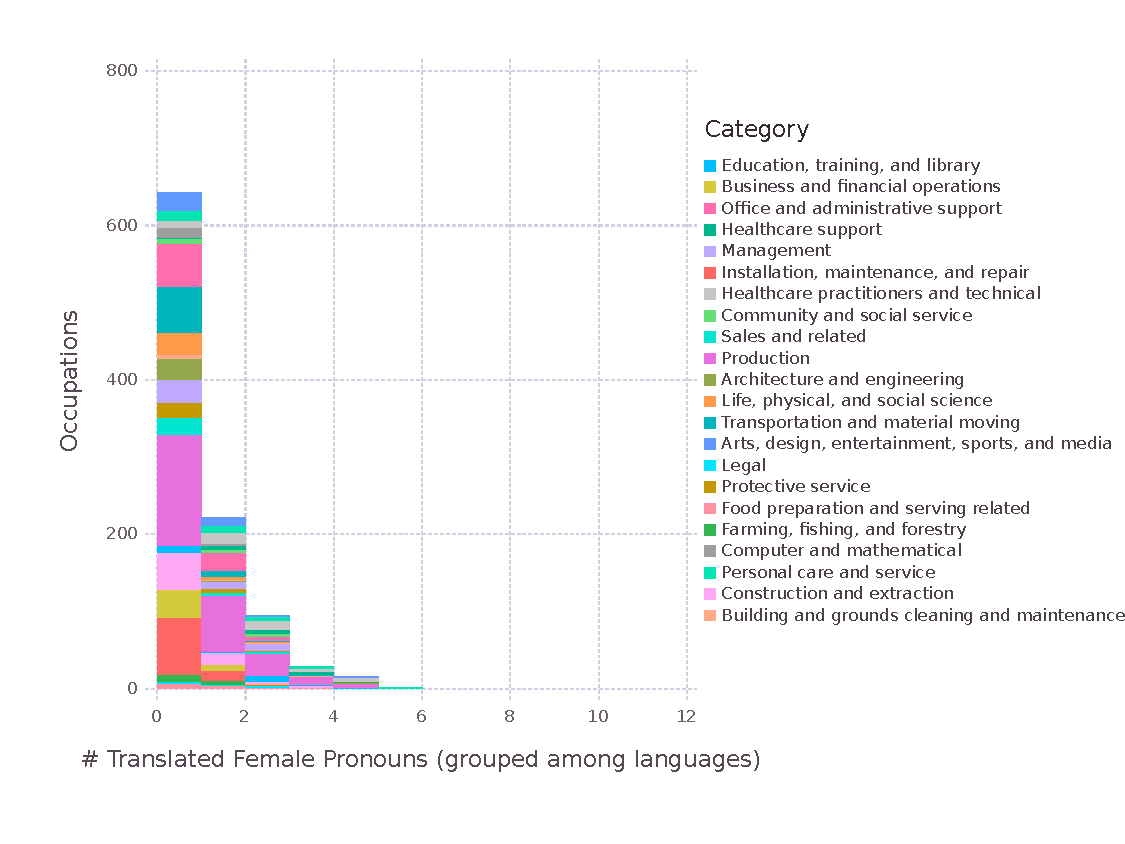
\includegraphics[width=10cm]{pictures/histogram-female}
	\caption{The data for the total number $X$ of female pronouns per occupation category suggests an inverse distribution. STEM fields such as life, social, computer and physical sciences, architecture, engineering and mathematics are nearly exclusively concentrated at $X=0$, while more evenly distributed fields such as production and healthcare (see Table \ref{tab:gender-by-category}) extend to higher values.}
	\label{fig:histogram-female}
\end{figure}

% Histogram with the distirbution of female pronouns for each occupation category (but categories are grouped into 'super-categories')
\begin{figure}[H]
	\centering
	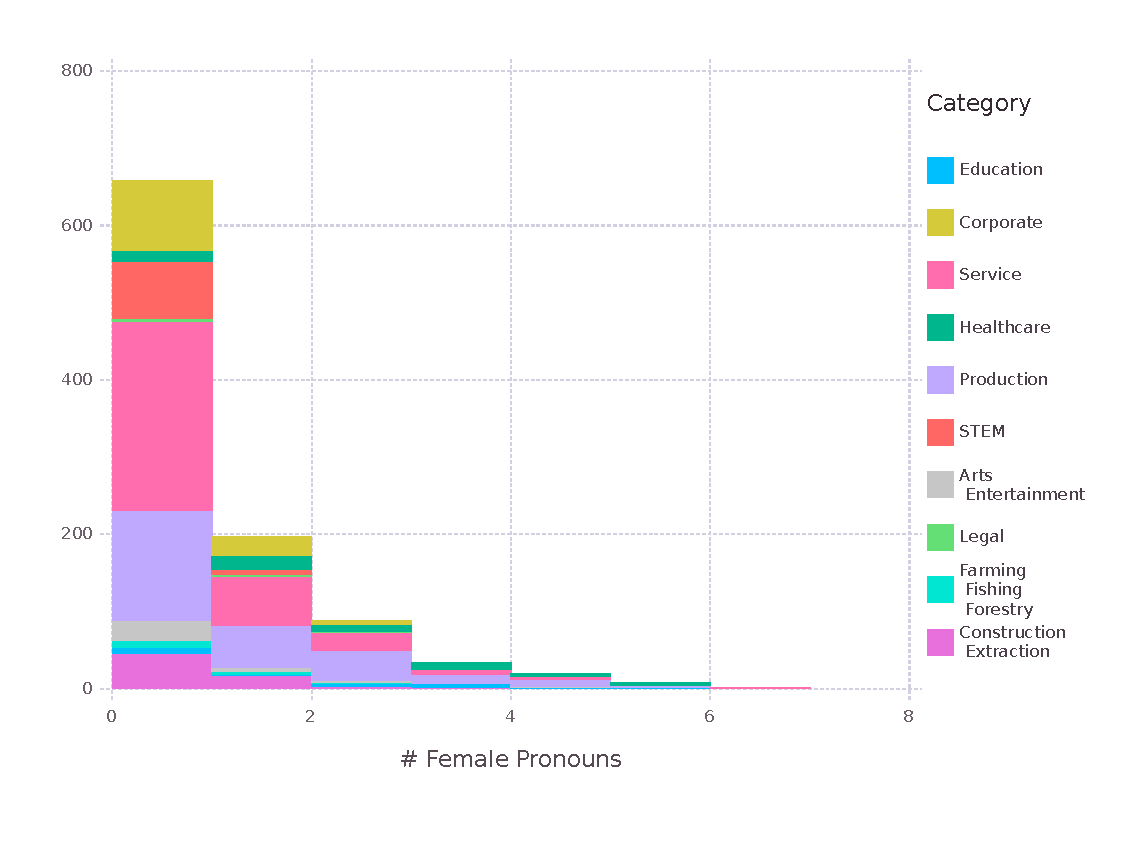
\includegraphics[width=10cm]{pictures/histogram-female-grouped}
	\caption{Coalescing the data from Table \ref{tab:gender-by-category} by grouping categories into broader groups helps us see how translated gender pronouns are distributed for some fields of interest such as STEM, Education, Arts / Entertainment, etc. In this context it becomes even clearer that STEM fields concentrate at $X = 0$, as discussed in Figure \ref{fig:histogram-female}.}
	\label{fig:histogram-female-grouped}
\end{figure}

% Histogram with the distirbution of male prononuns for each occupation category
\begin{figure}[H]
	\centering
	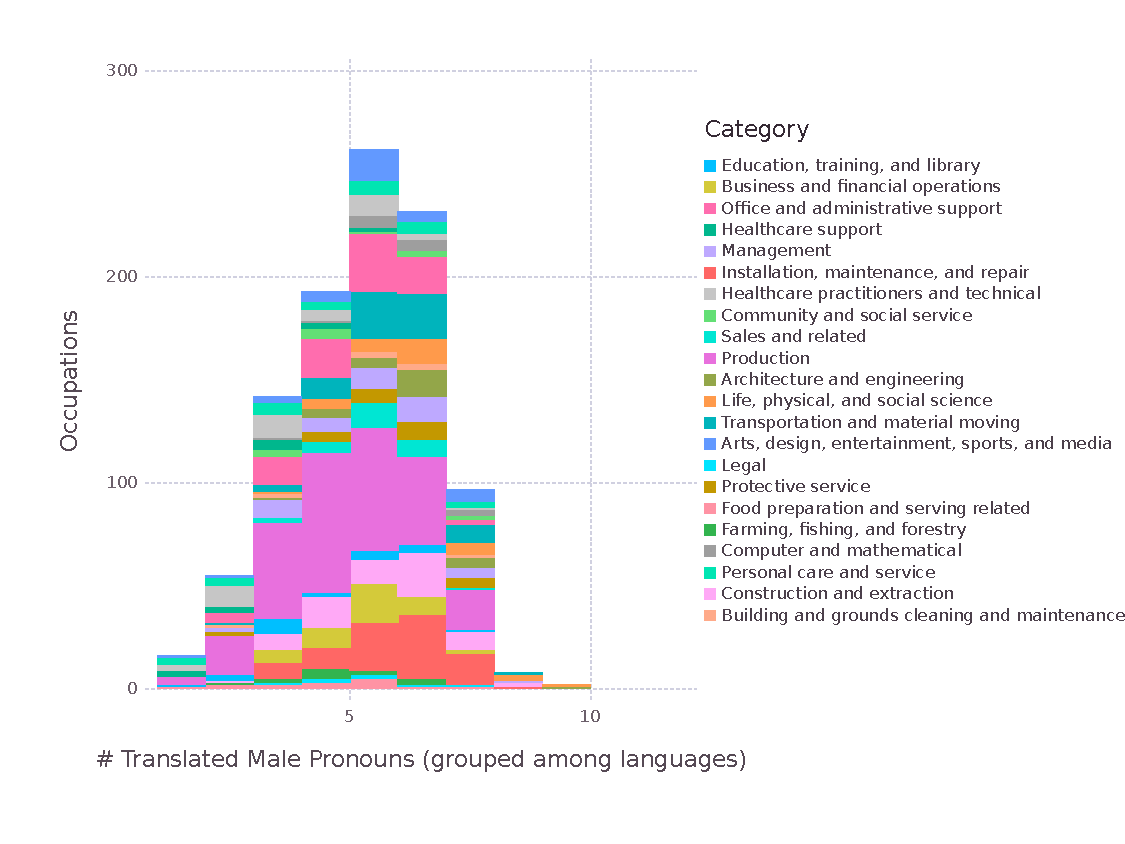
\includegraphics[width=10cm]{pictures/histogram-male}
	\caption{In contrast to female pronouns, male pronouns are seemingly skew normally distributed, with a peak at $X = 6$. One can see that STEM fields concentrate mainly to the right ($X \geq 6$).}
	\label{fig:histogram-male}
\end{figure}

% Histogram with the distirbution of male pronouns for each occupation category (but categories are grouped into 'super-categories')
\begin{figure}[H]
	\centering
	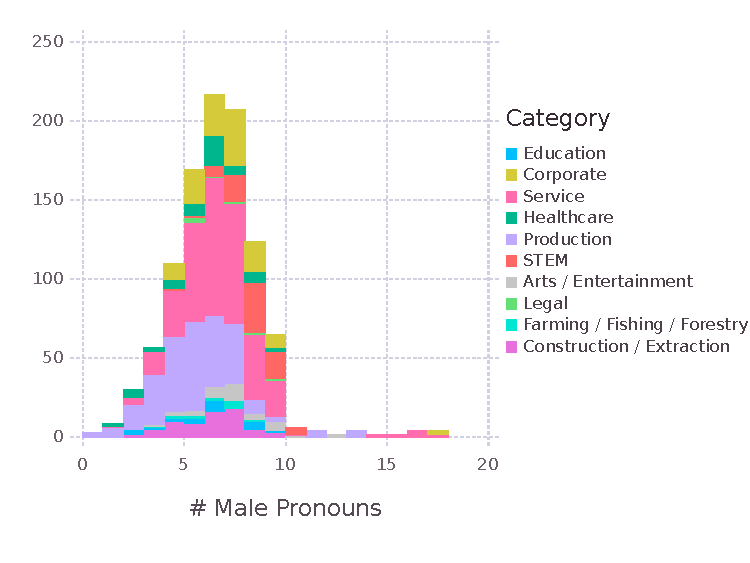
\includegraphics[width=10cm]{pictures/histogram-male-grouped}
	\caption{Coalescing the data from table \ref{tab:gender-by-category} by grouping categories into broader groups helps us see how translated gender pronouns are distributed for some fields of interest such as STEM, Education, Arts / Entertainment, etc. In this context it becomes clearer that STEM fields concentrate mainly to the right ($X \geq 6$), in contrast to what we observe for female pronouns (see Figure \ref{fig:histogram-female-grouped}).}
	\label{fig:histogram-male-grouped}
\end{figure}

% Histogram with the distribution of neutral pronouns for each occupation category
\begin{figure}[H]
	\centering
	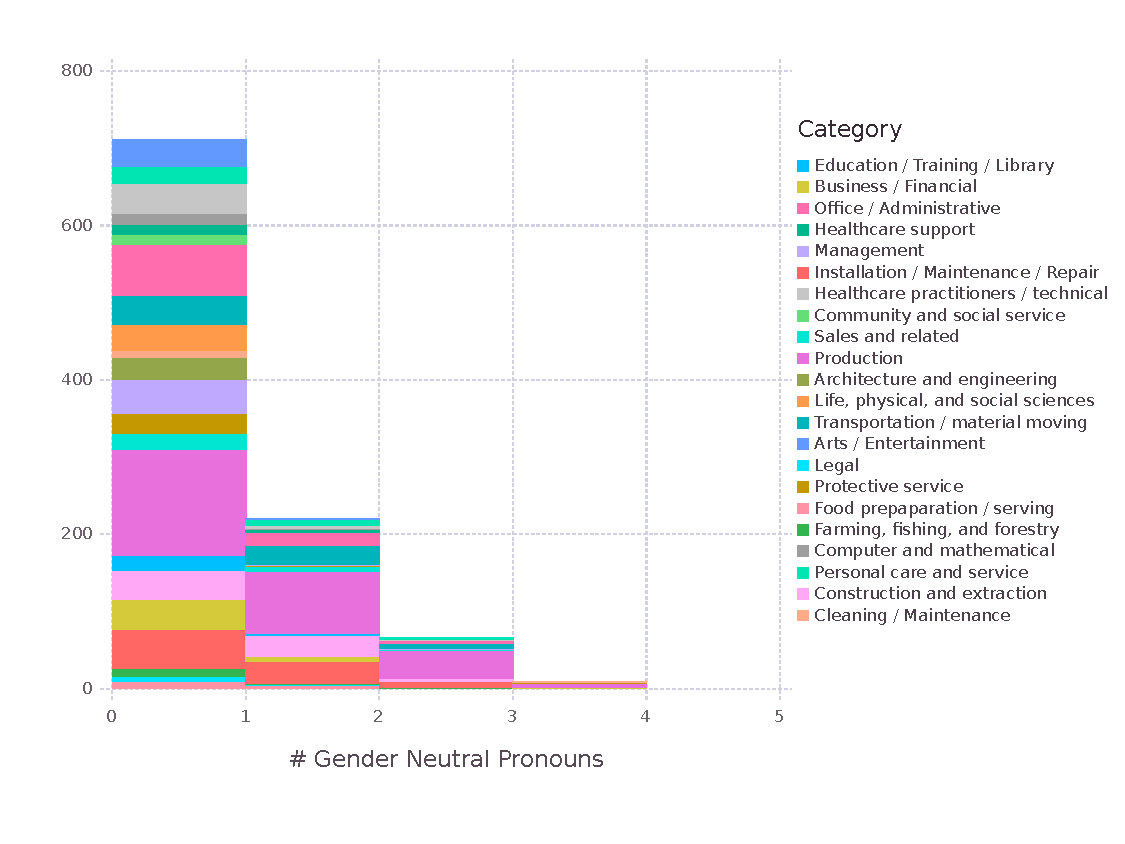
\includegraphics[width=10cm]{pictures/histogram-neutral}
	\caption{The scarcity of gender-neutral pronouns is manifest in their histogram, showing how they exceed the rarity even of female pronouns (see Figure \ref{fig:histogram-female}). Once again, STEM fields are predominantly concentrated on $X = 0$.}
	\label{fig:histogram-neutral}
\end{figure}

% Histogram with the distirbution of neutral pronouns for each occupation category (but categories are grouped into 'super-categories')
\begin{figure}[H]
	\centering
	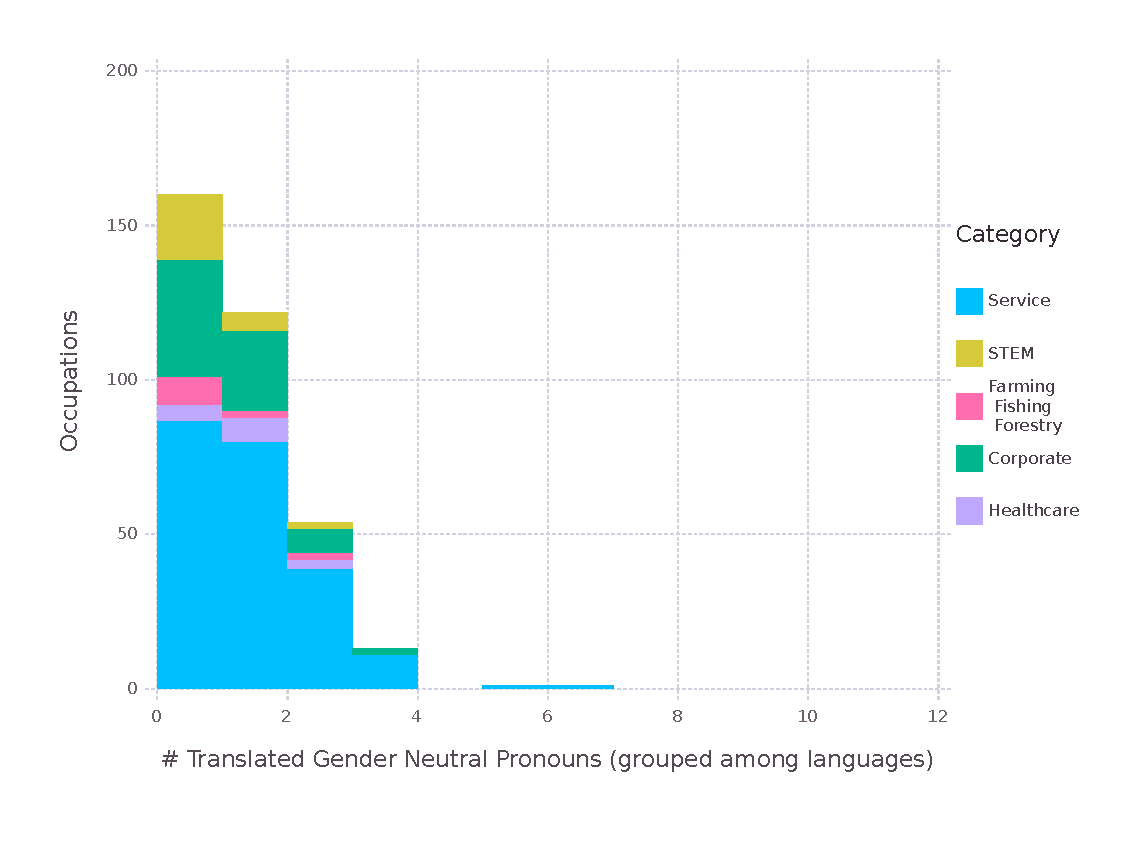
\includegraphics[width=10cm]{pictures/histogram-neutral-grouped}
	\caption{Coalescing the data from Table \ref{tab:gender-by-category} by grouping categories into broader groups helps us see how translated gender pronouns are distributed for some fields of interest such as STEM, Education, Arts / Entertainment, etc. Once again, STEM fields are predominantly concentrated at $X = 0$.}
	\label{fig:histogram-neutral-grouped}
\end{figure}

The barplots in Figure \ref{fig:gender-by-category} help us visualize how much of the distribution of each occupation category is composed of female, male and gender-neutral pronouns. In this context, STEM fields, which show a predominance of male defaults, are contrasted with healthcare and educations, which show a larger proportion of female pronouns.

% Barplot with % of female, male and neutral translated pronouns for each occupation category
\begin{figure}[H]
	\centering
	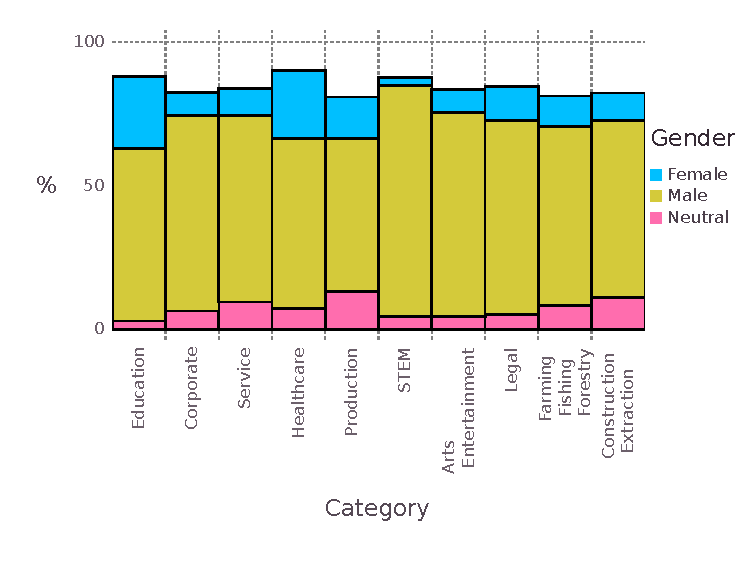
\includegraphics[width=10cm]{pictures/gender-by-category-grouped}
	\caption{Barplots show how much of the distribution of translated gender pronouns for each occupation category (grouped as in Table \ref{tab:gender-by-category-grouped}) is composed of female, male and neutral terms. STEM fields exhibit a predominance of male defaults and contrast with healthcare and education, with a larger proportion of female and neutral pronouns. Note that in general the bars do not add up to $100\%$, as there is a fair amount of translated sentences for which we cannot obtain a gender pronoun.}
	\label{fig:gender-by-category}
\end{figure}

\section{Distribution of translated gender pronouns per language}

We have taken the care of experimenting with a fair amount of different gender neutral languages. Because of that, another sensible way of coalescing our data is by language groups, as shown in Table \ref{tab:gender-by-language}. This can help us visualize the effect of different cultures in the genesis -- or lack thereof -- of gender bias. Nevertheless, the barplots in Figure \ref{fig:gender-by-language} are perhaps most useful to identifying the difficulty of extracting a gender pronoun when translating from certain languages. Japanese and Basque are good examples of this difficulty, although the quality of Turkish, Chinese and Yoruba translations are also compromised.

% Table with our gender bias results grouped by language
\begin{table}[H]
\small{
	\centering
	\begin{tabular}{|c|c|c|c|}
	\hline
	Language 	& Female ($\%$) 	& Male ($\%$)		& Neutral ($\%$)	\\ \hline
	\hline
	Malay     	& $4.122$ 			& $95.780$  		& $0.000$			\\ \hline
	Estonian  	& $18.351$			& $80.962$  		& $0.491$			\\ \hline
	Finnish   	& $33.562$			& $66.143$  		& $0.000$			\\ \hline
	Hungarian 	& $36.016$			& $63.297$  		& $0.393$			\\ \hline
	Armenian  	& $9.814$			& $81.256$  		& $0.589$			\\ \hline
	Japanese  	& $0.196$			& $26.791$  		& $1.079$			\\ \hline
	Turkish   	& $2.355$			& $63.199$  		& $18.449$			\\ \hline
	Yoruba    	& $1.178$			& $48.577$  		& $36.997$			\\ \hline
	Basque    	& $0.393$			& $12.365$  		& $34.838$			\\ \hline
	Swahili   	& $14.328$ 			& $85.574$  		& $0.000$			\\ \hline
	Chinese   	& $1.865$ 			& $69.382$  		& $9.225$			\\ \hline
	\end{tabular}
	\caption{Percentage of female, male and neutral gender pronouns obtained for each language, averaged over all occupations detailed in Table \ref{tab:gender-neutral-languages}. Note that columns do not in general add up to $100\%$, as there is a fair amount of translated sentences for which we cannot obtain a gender pronoun.}
	\label{tab:gender-by-language}
	}
\end{table}

% Barplot with % of female, male and neutral translated pronouns for each language
\begin{figure}[H]
	\centering
	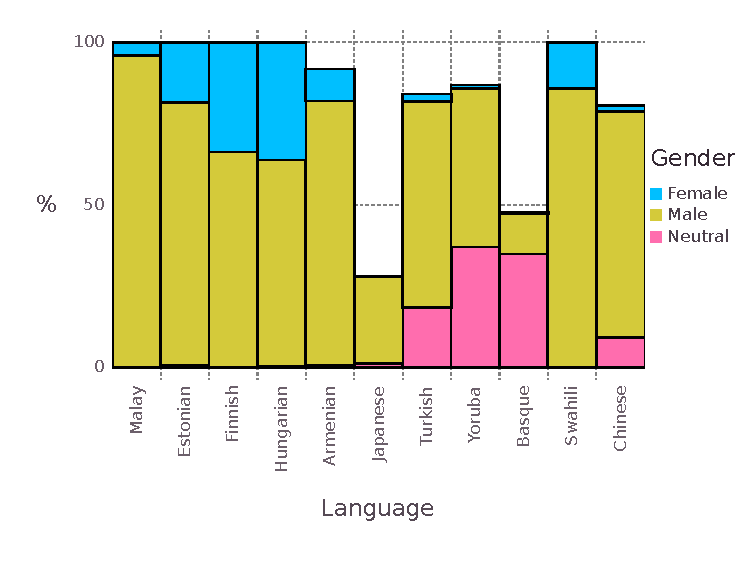
\includegraphics[width=10cm]{pictures/gender-by-language}
	\caption{The distribution of pronominal genders per language also suggests a tendency towards male defaults, with female pronouns reaching as low as $0.196\%$ and $1.865\%$ for Japanese and Chinese respectively. Once again not all bars add up to $100\%$ as Google Translate occasionally fails to translate sentences, particularly in Japanese and Basque. Among all tested languages, Basque was the only one to yield more gender neutral than male pronouns, with Yoruba and Turkish following after in this order.}
	\label{fig:gender-by-language}
\end{figure}

\section{Distribution of translated gender pronouns for varied adjectives}

Apart from occupations, which we have exhaustively examined by collecting labor data from the U.S. Bureau of Labor Statistics, we have also selected a small and for all purposes not representative subset of adjectives, in an attempt to provide preliminary evidence that the phenomenon of gender bias may extend beyond the professional context examined in this paper.

Once again the data points towards male defaults, but some variation can be observed throughout different adjectives. Sentences containing the words \emph{Shy}, \emph{Attractive}, \emph{Happy}, \emph{Kind} and \emph{Ashamed} are predominantly female translated (\emph{Attractive} is translated as female and gender-neutral in equal parts), while \emph{Arrogant}, \emph{Cruel} and \emph{Guilty} are disproportionately translated with male pronouns (\emph{Guilty} is in fact never translated with female or neutral pronouns).

% Table with our gender bias results for each adjective
\begin{table}[H]
\small{
	\centering
	\begin{tabular}{|c|c|c|c|c|}
	\hline
	Adjective 	& Female 	& Male 	& Neutral 	& Total 	\\ \hline
	\hline
	Happy		& $4$		& $3$	& $2$		& $11$		\\ \hline
	Wrong		& $0$		& $6$	& $4$		& $11$		\\ \hline
	Smart		& $2$		& $4$	& $3$		& $11$		\\ \hline
	Ashamed		& $3$		& $5$	& $1$		& $11$		\\ \hline
	Envious		& $2$		& $5$	& $1$		& $11$		\\ \hline
	Modest		& $1$		& $5$	& $3$		& $11$		\\ \hline
	Innocent	& $1$		& $7$	& $1$		& $11$		\\ \hline
	Sad			& $2$		& $5$	& $2$		& $11$		\\ \hline
	Afraid		& $1$		& $5$	& $0$		& $11$		\\ \hline
	Dumb		& $1$		& $5$	& $2$		& $11$		\\ \hline
	Kind		& $3$		& $3$	& $1$		& $11$		\\ \hline
	Loving		& $2$		& $5$	& $2$		& $11$		\\ \hline
	Arrogant	& $0$		& $8$	& $1$		& $11$		\\ \hline
	Helpless	& $2$		& $5$	& $2$		& $11$		\\ \hline
	Right		& $0$		& $6$	& $3$		& $11$		\\ \hline
	Brave		& $2$		& $6$	& $1$		& $11$		\\ \hline
	Proud		& $1$		& $7$	& $1$		& $11$		\\ \hline
	Cruel		& $1$		& $7$	& $2$		& $11$		\\ \hline
	Hateful		& $1$		& $4$	& $3$		& $11$		\\ \hline
	Guilty		& $0$		& $8$	& $0$		& $11$		\\ \hline
	Shy			& $5$		& $2$	& $2$		& $11$		\\ \hline
	Attractive	& $4$		& $1$	& $4$		& $11$		\\ \hline \hline
	Total 		& $38$		& $112$	& $41$		& -			\\ \hline 
	\end{tabular}
	\caption{Number of female, male and neutral pronominal genders in the translated sentences for each selected adjective.}
	\label{tab:gender-by-adjective}
	}
\end{table}

% Barplot with % of female, male and neutral translated pronouns for each adjective
\begin{figure}[H]
	\centering
	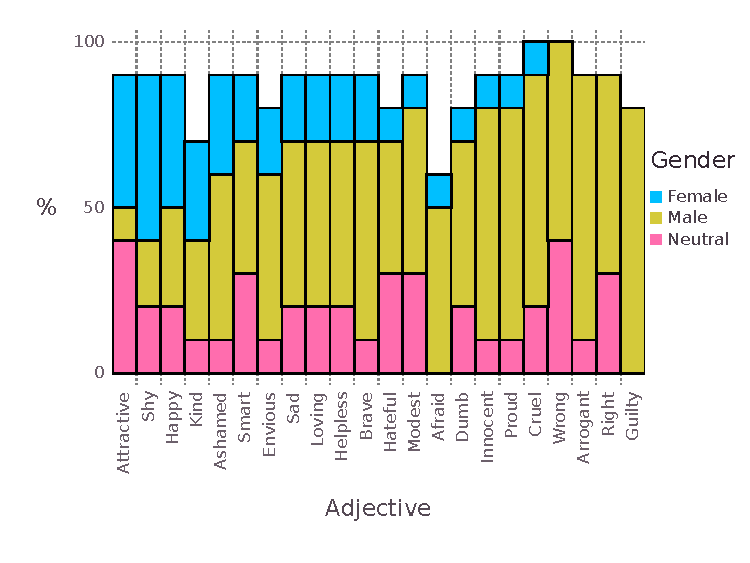
\includegraphics[width=10cm]{pictures/barplot-adjectives}
	\caption{The distribution of pronominal genders for each word in Table \ref{tab:adjectives} shows how stereotypical gender roles can play a part on the automatic translation of simple adjectives. One can see that adjectives such as \emph{shy} and \emph{attractive} are predominantly translated with female pronouns, while words like \emph{guilty}, \emph{innocent}, \emph{wrong}, \emph{right}, \emph{arrogant} are almost exclusively translated with male pronouns. Objective statements have a tendency towards male defaults, while statements concerning emotional states (\emph{shy}, \emph{happy}, \emph{kind}, \emph{ashamed}) amass at the other extreme of the sex ratio spectrum.}
	\label{fig:barplot-adjectives}
\end{figure}

\section{Comparison with women participation data across job positions}

A sensible objection to the conclusions we draw from our study is that the perceived gender bias in Google Translate results stems from the fact that (possibly) female participation in some job positions is itself low. We must account for the possibility that the statistics of gender pronouns in Google Translate outputs merely reflects a real-world asymmetry in the workplace. In this context, the argument in favor of a critical revision of statistic translation algorithms weakens considerably, and possibly shifts the blame away from these tools.

The U.S. Bureau of Labor Statistics data summarized in Table \ref{tab:occupations} contains statistics about the percentage of women participation in each occupation category. These data is also available for each individual occupation, which allows us to compute the frequency of women participation for each 12-quantile. We carried the same computation in the context of frequencies of translated female pronouns, and the resulting histograms are plotted side-by-side in Figure \ref{fig:histogram-compare-gt-real}. The data shows us that Google Translate outputs fail to follow the real-world distribution of female workers across a comprehensive set of job positions. The distribution of translated female pronouns is consistently inversely distributed, with female pronouns accumulating in the first 12-quantile. By contrast, BLS data shows that female participation peaks in the fourth 12-quantile and remains significant throughout the next ones.

% Histogram with the distirbution of male prononuns for each occupation category
\begin{figure}[H]
	\centering
	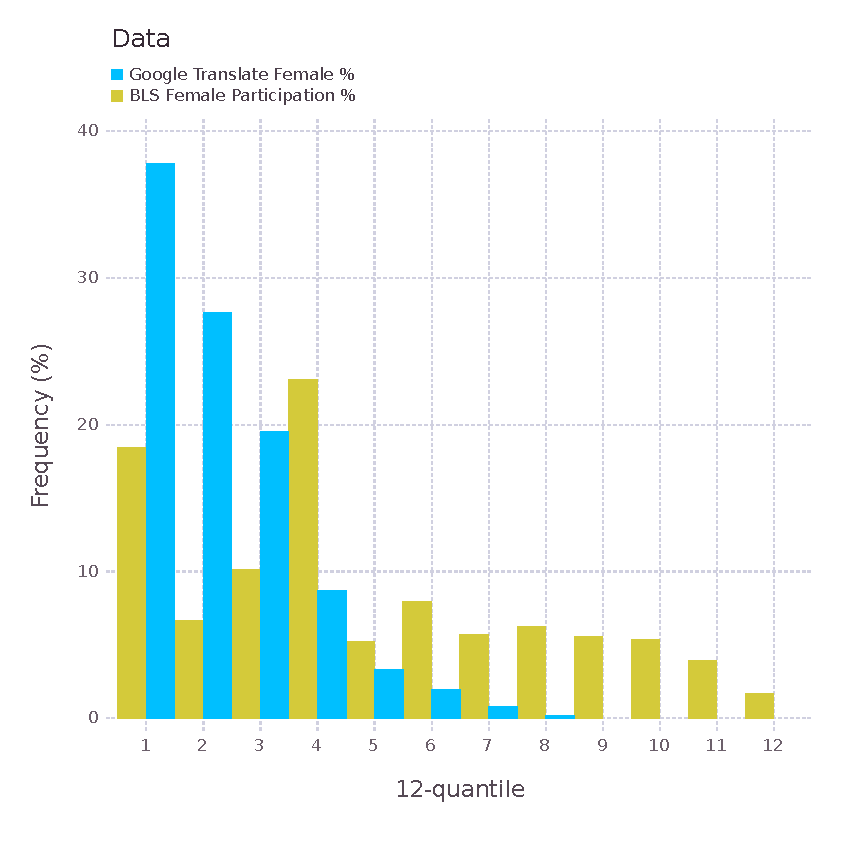
\includegraphics[width=10cm]{pictures/histogram-compare-gt-real}
	\caption{Women participation ($\%$) data obtained from the U.S. Bureau of Labor Statistics allows us to assess whether the Google Translate bias towards male defaults is at least to some extent explained by small frequencies of female workers in some job positions. Our data does not make a very good case for that hypothesis: the total frequency of translated female pronouns (in blue) for each 12-quantile (which is consistently inversely distributed) does not seem to respond to the higher proportion of female workers (in red) in the last quantiles. To remove doubt we have also plotted in yellow the frequency of translated female pronouns among male and female pronouns (i.e., excluding eventual translation errors and gender-neutral prononuns).}
	\label{fig:histogram-compare-gt-real}
\end{figure}

Running a t-test on the percentage of female translations over all translations for every occupation against the percentage of female participation in an occupation (surrogating with the LBS class value for the profession, in case it was missing), we see a mean of $11.11\%$ gender participation in the translations and a mean of $35.99\%$ in the LBS report. The variance reported for the translation results is also lower, at $\approx 0.01451$ in contrast with the report's $\approx 0.06668$. Altogether, the Pearson correlation between the two values is $\approx 0.30356$, with the p-values for one and two tail both being lower than the alpha value chosen ($\alpha = 0.05$). This result enforces the fact that the translation exhibits a tendency towards male defaults, even when the female participation in that job is higher than expected.

\ifx
\section{Results}

For each one of the tested 462 occupations (see Tables \ref{tab:occupations}, \ref{tab:occupations-examples}), we used the Python Google Translate API (\url{http://py-googletrans.readthedocs.io/en/latest/}) to translate sentences built with the templates in Table \ref{tab:templates} from each one of the tested languages in Table \ref{tab:gender-neutral-languages} to English. The resulting sentences are then classified as \emph{female}, \emph{male} or \emph{neutral} according to their respective pronouns. Sentences starting with \say{She/She's/Her} are classified as female, sentences starting with \say{He/He's/His} are classified as male and sentences starting with \say{It/It's/Its/They/They're/Their} are classified as (gender) neutral. The results from this analysis, which can be found in \url{https://github.com/marceloprates/Gender-Bias}, are further discussed below.

One can see either in Table \ref{tab:gender-by-category} or Figure \ref{fig:gender-by-category} that not only does Google Translate exhibit a tendency towards male defaults, but also that this tendency is further enhanced for typically male dominated fields such as computer science (with a ratio of $17.857$ male pronouns per female pronoun). Sentences about occupations from the \emph{Corporate} and \emph{Science} category are also disproportionately translated with male pronouns (sex ratios $9.444$ and $10.5$ respectively), while those containing occupations from the \emph{Dance} category achieve a sex ratio of almost one ($1.064$). Not one category has achieved a balanced sex ratio, neither does any category exhibit more gender neutral than male pronouns. In total, female pronouns add up to $16.522\%$ among all categories, while male pronouns add up to $63.083\%$ and gender neutral pronouns to just $7.912\%$, yielding an average sex ratio of $3.818$.

While grouping translations by category helps shed light on the stereotypical gender roles among different professions, grouping translations by language can help us understand the effect each culture possibly has on this issue. Table \ref{tab:gender-by-language} shows some sex ratios even larger than the previous ones, particularly when translating from Yoruba ($25.333$), Chinese ($27.5$) and Japanese, the last one peaking at an impressive ratio of $107.5$ male per female pronouns. Figure \ref{fig:gender-by-language} shows that, when grouping by language, gender neutral pronouns can be more prominent than male pronouns at least in one case: translating sentences from Basque yields 153 neutral vs 50 male and 5 female pronouns. Unfortunately this is the exception rather than the rule, with Yoruba following after with 131 neutral vs 304 male and 12 female pronouns. In total, female pronouns add up to $18.687\%$ among all categories, while male pronouns add up to $81.626\%$ and gender neutral pronouns to $8.466\%$, yielding an average sex ratio of $4.368$ ($14.405\%$ larger than what we get from grouping among categories). It should be noted however that Japanese and Basque, the two languages which stood out from the behavior observed in Figure \ref{fig:gender-by-category}, are precisely the two that Google Translate found hardest to translate. These findings should, as a result, be taken with a grain of salt.

% Table with our gender bias results grouped by language
\begin{table}[H]
\small{
	\centering
	\begin{tabular}{|c|c|c|c|}
	\hline
	Language 	& Female ($\%$) 	& Male ($\%$)		& Neutral ($\%$)	\\ \hline
	\hline
	Malay     	& $4.122$ 			& $95.780$  		& $0.000$			\\ \hline
	Estonian  	& $18.351$			& $80.962$  		& $0.491$			\\ \hline
	Finnish   	& $33.562$			& $66.143$  		& $0.000$			\\ \hline
	Hungarian 	& $36.016$			& $63.297$  		& $0.393$			\\ \hline
	Armenian  	& $9.814$			& $81.256$  		& $0.589$			\\ \hline
	Japanese  	& $0.196$			& $26.791$  		& $1.079$			\\ \hline
	Turkish   	& $2.355$			& $63.199$  		& $18.449$			\\ \hline
	Yoruba    	& $1.178$			& $48.577$  		& $36.997$			\\ \hline
	Basque    	& $0.393$			& $12.365$  		& $34.838$			\\ \hline
	Swahili   	& $14.328$ 			& $85.574$  		& $0.000$			\\ \hline
	Chinese   	& $1.865$ 			& $69.382$  		& $9.225$			\\ \hline \hline
	Total     	& ? 				& ? 				& ? 				\\ \hline
	\end{tabular}
	\caption{Number of female, male and neutral pronominal genders per language in the translated sentences. The corresponding sex ratios (\# Male / \# Female) show just how much male defaults are prominent in some languages such as Chinese, with almost 30 male pronouns for each female one.}
	\label{tab:gender-by-language}
	}
\end{table}

% Barplot with % of female, male and neutral translated pronouns for each language
\begin{figure}[H]
	\centering
	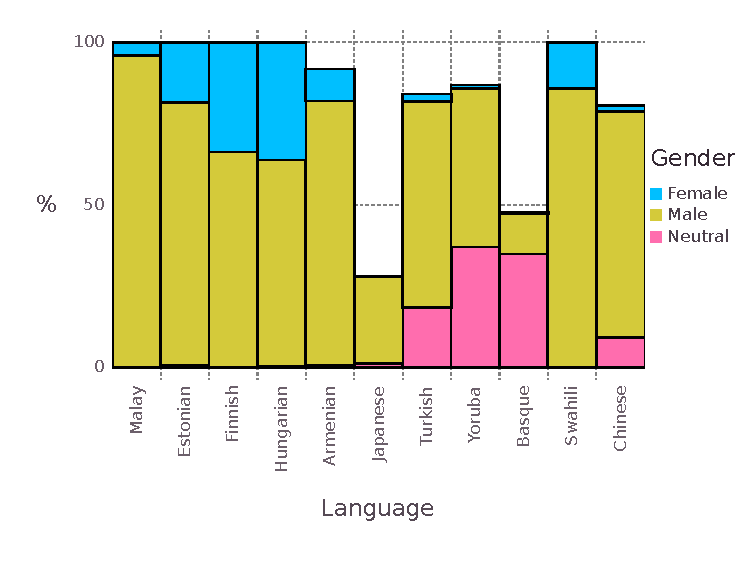
\includegraphics[width=10cm]{pictures/gender-by-language}
	\caption{The distribution of pronominal genders per language also suggests a tendency towards male defaults, with female pronouns reaching as low as $0.46\%$ and $2.98\%$ for Japanese and Chinese respectively. Once again not all bars add up to $100\%$ as Google Translate occasionally fails to translate sentences, particularly in Japanese and Basque. Among all tested languages, Basque was the only one to yield more gender neutral than male pronouns.}
	\label{fig:gender-by-language}
\end{figure}

Figures \ref{fig:histogram-female}, \ref{fig:histogram-male} and \ref{fig:histogram-neutral} shed further light on the asymmetry between the distribution male and female pronouns. While the number of occurrences of male pronouns tends towards a normal distribution, the figure changes drastically for the opposite gender, whose pronoun distribution is apparently governed by an inverse correlation. The behavior repeats itself for the gender neutral pronouns in Figure \ref{fig:histogram-neutral}.

Finally, Figure \ref{fig:barplot-adjectives} and Table \ref{tab:gender-by-adjective} show how stereotypical gender roles possibly play a part when simple adjectives are translated. We observed that objective statements such as \say{he/she is wrong/right/guilty/innocent} are biased towards male defaults, while statements concerning emotional states (\say{sad},\say{kind},\say{shy}) amass at the opposite extreme of the sex ratio spectrum. Unsurprisingly, the statement \say{he/she is attractive} is translated predominately with female pronouns.

% Table with our gender bias results for each adjective
\begin{table}[H]
\small{
	\centering
	\begin{tabular}{|c|c|c|c|c|c|}
	\hline
	Adjective 	& Female & Male & Neutral & Ratio & Total \\ \hline
	\hline
	Shy     	& 6  & 2   & 2  & 0.333 	& 12  \\ \hline
	Attractive 	& 4  & 2   & 4  & 0.500   	& 12  \\ \hline
	Happy   	& 5  & 3   & 2  & 0.600   	& 12  \\ \hline
	Kind    	& 4  & 3   & 1  & 0.750 	& 12  \\ \hline
	Ashamed 	& 4  & 5   & 1  & 1.250 	& 12  \\ \hline
	Smart   	& 2  & 5   & 3  & 2.500   	& 12  \\ \hline
	Envious 	& 2  & 6   & 1  & 3.000   	& 12  \\ \hline
	Sad     	& 2  & 6   & 2  & 3.000   	& 12  \\ \hline
	Loving  	& 2  & 6   & 2  & 3.000   	& 12  \\ \hline
	Helpless 	& 2  & 6   & 2  & 3.000   	& 12  \\ \hline
	Brave   	& 2  & 7   & 1  & 3.500   	& 12  \\ \hline
	Proud   	& 2  & 7   & 1  & 3.500   	& 12  \\ \hline
	Hateful 	& 1  & 5   & 3  & 5.000   	& 12  \\ \hline
	Dumb    	& 1  & 6   & 2  & 6.000   	& 12  \\ \hline
	Innocent 	& 1  & 8   & 1  & 8.000   	& 12  \\ \hline
	Right   	& 0  & 7   & 3  & -   		& 12  \\ \hline
	\hline
	Total   	& 43 & 129 & 41 & 3     	& 264 \\ \hline
	\end{tabular}
	\caption{Number of female, male and neutral pronominal genders in the translated sentences for each selected adjective.}
	\label{tab:gender-by-adjective}
	}
\end{table}

% Barplot with % of female, male and neutral translated pronouns for each adjective
\begin{figure}[H]
	\centering
	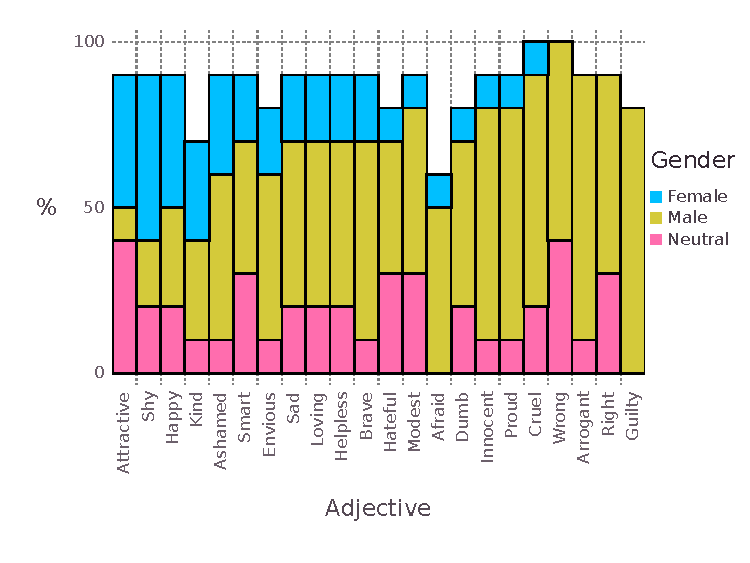
\includegraphics[width=10cm]{pictures/barplot-adjectives}
	\caption{The distribution of pronominal genders for each word in Table \ref{tab:adjectives} shows how stereotypical gender roles can play a part on the automatic translation of simple adjectives. One can see that adjectives such as \emph{shy} and \emph{attractive} are predominantly translated with female pronouns, while words like \emph{guilty}, \emph{innocent}, \emph{wrong}, \emph{right}, \emph{arrogant} are almost exclusively translated with male pronouns. Objective statements have a tendency towards male defaults, while statements concerning emotional states (\emph{shy}, \emph{happy}, \emph{kind}, \emph{ashamed}) amass at the other extreme of the sex ratio spectrum.}
	\label{fig:barplot-adjectives}
\end{figure}

\fi

\section{Conclusions}

In this paper, we have provided preliminary evidence that statistical translation tools such as Google Translate can exhibit gender biases and a strong tendency towards male defaults. Although implicit, these biases possibly stem from the real world data which is used to train them, and in this context possibly provide a window into the way our society talks (and writes) about women in the workplace. In this paper, we suggest that and test the hypothesis that statistical translation tools can be probed to yield insights about stereotypical gender roles in our society -- or at least in their training data. By translating professional-related sentences such as \say{He/She is an engineer} from gender neutral languages such as Hungarian and Chinese into  English, we were able to collect statistics bout the asymmetry between female and male pronominal genders in the translation outputs. Our results show that male defaults are not only prominent but exaggerated in fields suggested to be troubled with gender stereotypes, such as STEM (Science, Technology, Engineering and Mathematics) jobs. And Because Google Translate typically uses English as a \emph{lingua franca}
% PEDRO: reference?
to translate between other languages (e.g. Chinese $\rightarrow$ English $\rightarrow$ Portuguese), our findings possibly extend to translations between gender neutral languages and non-gender neutral languages (apart from English) in general, although we have not tested this hypothesis.

Although not conclusive, our results seem to suggest that this phenomenon extends beyond the scope of the workplace, with the proportion of female pronouns varying significantly according to adjectives used to describe a person. Adjectives such as \emph{Shy} and \emph{Attractive} are predominantly translated with female pronouns, while \emph{Guilty} and \emph{Cruel} are almost exclusively translated with male pronouns. Different languages also seemingly have a significant impact in machine gender bias, with Hungarian exhibiting a better equilibrium between male and female pronouns than for example Chinese. Some languages such as Yoruba and Basque were found to translate sentences with gender neutral pronouns very often, although this is the exception rather than the rule and these languages also exhibit a high frequency of translation errors.

To solidify our results, we ran our pronominal gender translation statistics against the U.S. Bureau of Labor Statistics data on the frequency of women participation for each job position. Although Google Translate exhibits male defaults, this phenomenon may merely reflect the unequal distribution of male and female workers in some job positions. To test this hypothesis, we compared the distribution of female workers with the frequency of female translations, finding no correlation between said variables. Our data shows that Google Translate outputs fail to reflect the real-world distribution of female workers, under-estimating the expected frequency. That is to say that even if we do not expect a 50:50 distribution of translated gender pronouns, Google Translate exhibits male defaults in a greater frequency that job occupation data alone would suggest. The prominence of male defaults in Google Translate is therefore to the best of our knowledge yet lacking a clear justification.

We think this work can shed further light on what we believe is a pressing ethical difficulty arising from modern statistical machine translation, and hope that it will lead to discussions about the role of AI engineers on minimizing potential harmful effects of the pressing modern concerns of machine bias. We are optimistic that unbiased results can be obtained with little effort and marginal cost to the performance of current methods, to which current \emph{debiasing} algorithms in the scientific literature are a testament.

\bibliography{main}



\end{document}N

\begin{thebibliography}{xx}

\harvarditem[Angwin et~al.]{Angwin, Larson, Mattu \harvardand\
  Kirchner}{2016}{angwin2016machine}
Angwin, J., Larson, J., Mattu, S. \harvardand\ Kirchner, L.  \harvardyearleft
  2016\harvardyearright , `Machine bias: {T}here's software used across the
  country to predict future criminals and it's biased against blacks'.
\newblock Last visited 2017-12-17.
\newline\harvardurl{https://www.
  propublica.org/article/machine-bias-risk-assessments-in-criminal-sentencing}

\harvarditem[Bahdanau et~al.]{Bahdanau, Cho \harvardand\
  Bengio}{2014}{Bahdanau2014}
Bahdanau, D., Cho, K. \harvardand\ Bengio, Y.  \harvardyearleft
  2014\harvardyearright , `Neural machine translation by jointly learning to
  align and translate', {\em CoRR} {\bf abs/1409.0473}.
\newline\harvardurl{http://arxiv.org/abs/1409.0473}

\harvarditem[Bolukbasi et~al.]{Bolukbasi, Chang, Zou, Saligrama \harvardand\
  Kalai}{2016}{bolukbasi2016man}
Bolukbasi, T., Chang, K.-W., Zou, J.~Y., Saligrama, V. \harvardand\ Kalai,
  A.~T.  \harvardyearleft 2016\harvardyearright , Man is to computer programmer
  as woman is to homemaker? debiasing word embeddings, {\em in} `Advances in
  Neural Information Processing Systems', pp.~4349--4357.

\harvarditem{Carl \harvardand\ Way}{2003}{carl2003recent}
Carl, M. \harvardand\ Way, A.  \harvardyearleft 2003\harvardyearright , {\em
  Recent advances in example-based machine translation}, Vol.~21, Springer
  Science \& Business Media.

\harvarditem{Chomsky}{2011}{Chomsky2011}
Chomsky, N.  \harvardyearleft 2011\harvardyearright , `The golden age: A look
  at the original roots of artificial intelligence, cognitive science, and
  neuroscience (partial transcript of an interview with {N}. {C}homsky at
  {MIT150} {S}ymposia: Brains, minds and machines symposium'.
\newblock Last visited 2017-12-26.
\newline\harvardurl{https://chomsky.info/20110616/}

\harvarditem{Dascal}{1982}{dascal1982universal}
Dascal, M.  \harvardyearleft 1982\harvardyearright , `Universal language
  schemes in {E}ngland and {F}rance, 1600-1800 comments on {J}ames {K}nowlson',
  {\em Studia leibnitiana} {\bf 14}(1),~98--109.

\harvarditem[Firat et~al.]{Firat, Cho, Sankaran, Yarman{-}Vural \harvardand\
  Bengio}{2017}{Firat2017}
Firat, O., Cho, K., Sankaran, B., Yarman{-}Vural, F.~T. \harvardand\ Bengio, Y.
   \harvardyearleft 2017\harvardyearright , `Multi-way, multilingual neural
  machine translation', {\em Computer Speech {\&} Language} {\bf 45},~236--252.
\newline\harvardurl{https://doi.org/10.1016/j.csl.2016.10.006}

\harvarditem{Garcia}{2016}{garcia2016racist}
Garcia, M.  \harvardyearleft 2016\harvardyearright , `Racist in the machine:
  The disturbing implications of algorithmic bias', {\em World Policy Journal}
  {\bf 33}(4),~111--117.

\harvarditem{Gordin}{2015}{gordin2015scientific}
Gordin, M.~D.  \harvardyearleft 2015\harvardyearright , {\em Scientific Babel:
  How science was done before and after global English}, University of Chicago
  Press.

\harvarditem[Hajian et~al.]{Hajian, Bonchi \harvardand\
  Castillo}{2016}{hajian2016algorithmic}
Hajian, S., Bonchi, F. \harvardand\ Castillo, C.  \harvardyearleft
  2016\harvardyearright , Algorithmic bias: From discrimination discovery to
  fairness-aware data mining, {\em in} `Proceedings of the 22nd ACM SIGKDD
  international conference on knowledge discovery and data mining', ACM,
  pp.~2125--2126.

\harvarditem{Hutchins}{1986}{hutchins1986machine}
Hutchins, W.~J.  \harvardyearleft 1986\harvardyearright , {\em Machine
  translation: past, present, future}, Ellis Horwood Chichester.

\harvarditem[Johnson et~al.]{Johnson, Schuster, Le, Krikun, Wu, Chen, Thorat,
  Vi{\'{e}}gas, Wattenberg, Corrado, Hughes \harvardand\
  Dean}{2017}{wu2016google}
Johnson, M., Schuster, M., Le, Q.~V., Krikun, M., Wu, Y., Chen, Z., Thorat, N.,
  Vi{\'{e}}gas, F.~B., Wattenberg, M., Corrado, G., Hughes, M. \harvardand\
  Dean, J.  \harvardyearleft 2017\harvardyearright , `Google's multilingual
  neural machine translation system: Enabling zero-shot translation', {\em
  {TACL}} {\bf 5},~339--351.
\newline\harvardurl{https://transacl.org/ojs/index.php/tacl/article/view/1081}

\harvarditem{Kelman}{2014}{TranslateCommunity}
Kelman, S.  \harvardyearleft 2014\harvardyearright , `Translate community: Help
  us improve google translate!'.
\newblock Last visited 2018-3-12.
\newline\harvardurl{https://search.googleblog.com/2014/07/translate-community-help-us-improve.html}

\harvarditem{Kirkpatrick}{2016}{kirkpatrick2016battling}
Kirkpatrick, K.  \harvardyearleft 2016\harvardyearright , `Battling algorithmic
  bias: how do we ensure algorithms treat us fairly?', {\em Communications of
  the ACM} {\bf 59}(10),~16--17.

\harvarditem{Koehn}{2009}{koehn2009statistical}
Koehn, P.  \harvardyearleft 2009\harvardyearright , {\em Statistical machine
  translation}, Cambridge University Press.

\harvarditem[Koehn et~al.]{Koehn, Hoang, Birch, Callison{-}Burch, Federico,
  Bertoldi, Cowan, Shen, Moran, Zens, Dyer, Bojar, Constantin \harvardand\
  Herbst}{2007}{Moses2007}
Koehn, P., Hoang, H., Birch, A., Callison{-}Burch, C., Federico, M., Bertoldi,
  N., Cowan, B., Shen, W., Moran, C., Zens, R., Dyer, C., Bojar, O.,
  Constantin, A. \harvardand\ Herbst, E.  \harvardyearleft
  2007\harvardyearright , Moses: Open source toolkit for statistical machine
  translation, {\em in} `{ACL} 2007, Proceedings of the 45th Annual Meeting of
  the Association for Computational Linguistics, June 23-30, 2007, Prague,
  Czech Republic'.
\newline\harvardurl{http://aclweb.org/anthology/P07-2045}

\harvarditem{Locke \harvardand\ Booth}{1955}{locke1955machine}
Locke, W.~N. \harvardand\ Booth, A.~D.  \harvardyearleft 1955\harvardyearright
  , {\em Machine translation of languages: fourteen essays}, Published jointly
  by Technology Press of the Massachusetts Institute of Technology and Wiley,
  New York.

\harvarditem{Mills}{2017}{racistsoapdispenser2017}
Mills, K.-A.  \harvardyearleft 2017\harvardyearright , `'{R}acist' soap
  dispenser refuses to help dark-skinned man wash his hands - but {T}witter
  blames 'technology''.
\newblock Last visited 2017-12-17.
\newline\harvardurl{http://www.mirror.co.uk/news/world-news/racist-soap-dispenser-refuses-help-11004385}

\harvarditem{Norvig}{2017}{norvig2017chomsky}
Norvig, P.  \harvardyearleft 2017\harvardyearright , `On {C}homsky and the two
  cultures of statistical learning'.
\newblock Last visited 2017-12-17.
\newline\harvardurl{http://norvig.com/chomsky.html}

\harvarditem{Olson}{2018}{AlgorithmGtranslateSexist2018}
Olson, P.  \harvardyearleft 2018\harvardyearright , `The algorithm that helped
  google translate become sexist'.
\newblock Last visited 2018-3-12.
\newline\harvardurl{https://www.forbes.com/sites/parmyolson/2018/02/15/the-algorithm-that-helped-google-translate-become-sexist/\#1c1122c27daa}

\harvarditem{Papenfuss}{2017}{womanunlockphone2017}
Papenfuss, M.  \harvardyearleft 2017\harvardyearright , `Woman in {C}hina says
  colleague's face was able to unlock her i{P}hone {X}'.
\newblock Last visited 2017-12-17.
\newline\url{http://www.huffpostbrasil.com/entry/iphone-face-recognition-double_us_5a332cbce4b0ff955ad17d50}

\harvarditem{Schiebinger}{2014}{schiebinger2014scientific}
Schiebinger, L.  \harvardyearleft 2014\harvardyearright , `Scientific research
  must take gender into account', {\em Nature} {\bf 507}(7490),~9.

\harvarditem{Shankland}{2017}{Gtranslate200daily2017}
Shankland, S.  \harvardyearleft 2017\harvardyearright , `Google translate now
  serves 200 million people daily'.
\newblock Last visited 2018-3-12.
\newline\harvardurl{https://www.cnet.com/news/google-translate-now-serves-200-million-people-daily/}

\harvarditem{Wang \harvardand\ Kosinski}{2017}{wang2017deep}
Wang, Y. \harvardand\ Kosinski, M.  \harvardyearleft 2017\harvardyearright ,
  `Deep neural networks are more accurate than humans at detecting sexual
  orientation from facial images'.

\harvarditem{Weaver}{1955}{weaver1955translation}
Weaver, W.  \harvardyearleft 1955\harvardyearright , Translation, {\em in}
  W.~N. Locke \harvardand\ A.~D. Booth, eds, `Machine translation of
  languages', Vol.~14, Cambridge: Technology Press, MIT, pp.~15--23.
\newblock Last visited 2017-12-17.
\newline\harvardurl{http://www.mt-archive.info/Weaver-1949.pdf}

\end{thebibliography}
